%%%%%%%%%%%%%%%%%%%%%%%%%%%%%%%%%%%%%%%%%
% University Assignment Title Page 
% LaTeX Template
% Version 1.0 (27/12/12)
%
% This template has been downloaded from:
% http://www.LaTeXTemplates.com
%
% Original author:
% WikiBooks (http://en.wikibooks.org/wiki/LaTeX/Title_Creation)
%
% License:
% CC BY-NC-SA 3.0 (http://creativecommons.org/licenses/by-nc-sa/3.0/)
% 
% Instructions for using this template:
% This title page is capable of being compiled as is. This is not useful for 
% including it in another document. To do this, you have two options: 
%
% 1) Copy/paste everything between \begin{document} and \end{document} 
% starting at \begin{titlepage} and paste this into another LaTeX file where you 
% want your title page.
% OR
% 2) Remove everything outside the \begin{titlepage} and \end{titlepage} and 
% move this file to the same directory as the LaTeX file you wish to add it to. 
% Then add \input{./title_page_1.tex} to your LaTeX file where you want your
% title page.
%
%%%%%%%%%%%%%%%%%%%%%%%%%%%%%%%%%%%%%%%%%
%\title{Title page with logo}
%----------------------------------------------------------------------------------------
%	PACKAGES AND OTHER DOCUMENT CONFIGURATIONS
%----------------------------------------------------------------------------------------

\documentclass[12pt]{report}
\usepackage[english]{babel}
\usepackage{apacite}
\usepackage[utf8x]{inputenc}
\usepackage{geometry}
	\geometry{
		a4paper,
		total = {160mm, 245mm},
		left = 30mm,
		top = 30mm
	}
\usepackage[super,sort]{natbib}
\usepackage{tgbonum}
\usepackage{amsmath}
\usepackage{graphicx}
\graphicspath{{images/}}
\usepackage[colorinlistoftodos]{todonotes}

\begin{document}

\begin{titlepage}

\newcommand{\HRule}{\rule{\linewidth}{0.5mm}} % Defines a new command for the horizontal lines, change thickness here

\center % Center everything on the page
 
%----------------------------------------------------------------------------------------
%	HEADING SECTIONS
%----------------------------------------------------------------------------------------

\textsc{\LARGE Northeastern University}\\[1.5cm] % Name of your university/college
\textsc{\Large Master's Thesis Proposal}\\[0.5cm] % Major heading such as course name
\textsc{\large CS 7990}\\[0.5cm] % Minor heading such as course title

%----------------------------------------------------------------------------------------
%	TITLE SECTION
%----------------------------------------------------------------------------------------

\HRule \\[0.4cm]
{\Large \bfseries Word-vector Regularizer of synonymous but rare words in the Bag-of-Words model for Classification Problems}\\[0.4cm] % Title of your document
\HRule \\[1.5cm]
 
%----------------------------------------------------------------------------------------
%	AUTHOR SECTION
%----------------------------------------------------------------------------------------

\begin{minipage}{0.4\textwidth}
\begin{flushleft} \large
\emph{Author:}\\
Ramkishan \textsc{Panthena} % Your name
\end{flushleft}
\end{minipage}
~
\begin{minipage}{0.4\textwidth}
\begin{flushright} \large
\emph{Advisor:} \\
Dr. Virgil \textsc{Pavlu} % Supervisor's Name
\end{flushright}
\end{minipage}\\[2cm]

% If you don't want a supervisor, uncomment the two lines below and remove the section above
%\Large \emph{Author:}\\
%John \textsc{Smith}\\[3cm] % Your name

%----------------------------------------------------------------------------------------
%	DATE SECTION
%----------------------------------------------------------------------------------------

{\large \today}\\[2cm] % Date, change the \today to a set date if you want to be precise

%----------------------------------------------------------------------------------------
%	LOGO SECTION
%----------------------------------------------------------------------------------------


\includegraphics[width=4cm, height=4cm]{logo.jpg}\\[1cm] % Include a department/university logo - this will require the graphicx package
 
%----------------------------------------------------------------------------------------

%\vfill % Fill the rest of the page with whitespace

\end{titlepage}


\begin{abstract}
A simple and efficient baseline for text classification is to represent sentences as bag-of-words (BoW) and train a linear classifier. The bag-of-words model is simple to implement and offers flexibility for customization by providing different scoring techniques for user specific text data.

However, a large vocabulary can cause extremely sparse representations which are harder to model, where the challenge is for models to harness very little information in such a large representational space. In such cases, the traditional logistic regression model would treat each word separately and assign them different coefficients based on the frequency in which they occur in the train set. This would result in lower test accuracy as it comes across instances where a word which was occurring less frequently in the train set, occurs more often in the test set.

In this work, we are proposing a novel regularizer that would assign similar weights to words with nearly the same meaning. This will be achieved by training a neural network model by making the regression co-efficient of a word to be a function of its word-vector representation. Thus, based on how similar two features are, our proposed model can improve the feature importance of a sparse word by increasing its regression co-efficient, thereby improving the test accuracy in the above mentioned scenario.

\end{abstract}

\chapter{Introduction}

The goal of text classification is to classify text documents into one or more classes according to their content. For this purpose, a document must be transformed into a representation which is suitable for the learning algorithm and the classification task. Representing documents as bag-of-words is a commonly used method in document classification where the frequency of occurrence of each word is used as a feature for training a classifier. However, one should note that when using this representation, some document information is lost as the model disregards grammar and word ordering.

\section{Problem Statement}

Although the bag-of-words model is widely used and performs exceptionally well in most text classification problems, it contains several limitations. As per Zipf's law \cite{li1992random}, given a large sample of words used, the frequency of any word is inversely proportional to its rank in the frequency table. So, word number n has a frequency proportional to 1/n. Thus, a large vocabulary can cause extremely sparse representations. 

The classification accuracy we observe on the test set largely depends on the quality of training sets we have used to build our models. That is, if the training information is sparse, then we can expect the category model to be a poor representation of a category thereby leading to poor classification accuracy. Words that occur rarely do not give a learning algorithm enough information to determine its influence on classification correctly.

Thus, in such a case the traditional logistic regression model would treat each word separately and assign them different coefficients based on the effect of the feature on the response variable. As the training data for these rare words would be sparse, their coefficients would be near 0 implying that the effect of these features is small. This may not be the case as these rare words might be misrepresented due to sparse data. Our model tries to solve this problem by using a word-vector regularizer that assigns similar coefficients to words which are used in a similar context, thereby boosting the effect of similar but rare features on the final prediction.

\chapter{Related work}

A number of approaches have been proposed to increase the classification accuracy on the bag-of-words model.

To aggressively reduce the dimensionality of models, Joachims \cite{joachims1996probabilistic} (1996), Yang and Pedersen\cite{yang1997comparative} (1997) suggested pruning of infrequent words. Mansuy and Hilder \cite{mansuy2006characterization} (2006) recommended removing of stop words and part-of-speech tags. Porter \cite{porter1980algorithm} (1980) proposed removal of suffixes from words. Quinlan \cite{quinlan2014c4} (1993) suggested choosing words which have high mutual information with the target concept.

In an attempt to address the issue of related concepts in text classification, many researchers have incorporated features using dictionaries and encyclopedias. Mavroeidis et. al \cite{mavroeidis2005word} (2005) proposed to extend the traditional bag of words representation by incorporating syntactic and semantic relationships among words using a Word Sense Disambiguation approach. Wang and Domeniconi \cite{wang2008building} (2008) explored a similar approach by embedding background knowledge derived from Wikipedia to enrich the representation of documents. Recently, Heal et. al \cite{heap2017word} (2017) introduced a method for enriching the bag-of-words model by complementing rare term information with related terms from Word Vector models.

In addition to incorporating related concepts to improve classification performance, other approaches have also been proposed. One of these approaches considers using part-of-speech tags associated with words contained in a document (Scott and Matwin \cite{scott1998text} 1998), (Jensen and Martinez \cite{jensen2000improving} 2000). Since words can have multiple meanings depending upon how and where they are used in a sentence, the part-of-speech may be relevant to text classification.

\chapter{Proposed Method}

In this method, we propose to enhance the bag-of-words model for text classification by presenting a novel regularizer which would assign similar coefficients to words used in similar context.

\section{Logistic Regression model}

Formally, the problem we are trying to solve can be formulated as follows: Given a set of m documents with n features, the documents would be represented by matrix X $\in$ R$^{m x n}$. For the $i^{th}$ document $x^{(i)}$, with $y^{(i)}$ as its output variable, the hypothesis function for the logistic regression model is given by:

\begin{equation}
h(x^{(i)}) = \sigma(\theta^{T}x^{(i)} + b)
\end{equation}

where $i$ is the $i^{th}$ document, and $\theta$ and $b$ are the parameters we need to learn so that $h(x)$ is approximately equal to the target $y$.

%\vspace{5mm}

\section{Our model}

In case of our model, the parameter $\theta$ would now be a function of a d-dimensional word-vector of its corresponding feature $x_{k}$. These features will be regulated by a separate set of weights $w$ which need to be learned. Thus, the parameter $\theta_{k}$ for a feature $x_{k}$ would be represented as:

\begin{equation}
\theta_{k} = w^{T} wordvector(x_{k})
\end{equation}

The $\theta$ for an entire document $x^{(i)}$ would be:

\begin{equation}
\theta = \sum_{j=1}^{n}{w^{T} wordvector(x_{j})}
\end{equation}

Thus, the hypothesis and cost function for our word-vector model would be given as:

\begin{equation}
h(x^{(i)}) = \sigma{((\sum_{j=1}^{n}{w^{T} wordvector(x_{j})})^{(i)}+b)}
\end{equation}

\begin{equation}\label{cost_fn_eq}
Cost(h_{\theta}(x), y) = 
\begin{cases}
-log(h_{\theta}(x)), $\qquad if y=1$
\\
-log(1-h_{\theta}(x)), $ if y=0$
\end{cases}
\end{equation}

Since words used in similar context will have similar word-vectors and by making the regression co-efficient of a word to be a function of its word-vector representation, the hypothesis is that we can regularize the regression co-efficients of two similar words to have similar values. So, if one word occurs more frequently and has higher regression co-efficient, the other word even if it is very rare would be considered an important feature and would have higher a regression co-efficient. This would improve the classification performance in cases where these rare words occur more frequently in the test set.

\vspace{5mm}

Both the logistic regression and our proposed model can be visualized through the network illustration in Fig ().

\section{Implementation}

\subsection{Obtain word-vectors}

Out of the successful deep learning models used for word-embeddings, two of the most popular ones are Word2Vec \cite{le2014distributed} and Global Vectors \cite{pennington2014glove}. For our research, we will be using Google's Word2Vec which has pre-trained word-vectors with 300 dimensions trained using over 100 billion words. 

For larger datasets having vocabulary outside of Google's pre-trained word-vectors and having a fairly different context than that was used by Google's model, the word-vectors should be re-trained on the training data.

\subsection{Train new model}

Once the features have been extracted using the bag-of-words model and their corresponding word-vectors obtained, we can train a neural network model based on the cost function in (\ref{cost_fn_eq})

\chapter{Experiments}

\section{Baseline}

We compare our model to the vanilla logistic regression algorithm by implementing both using the TensorFlow library. Both the models can perform multi-class and multi-label classification. For multi-class, we use the softmax function to assign probabilities to each class which add up to 1. We use the sigmoid function for multi-label classification to train an independent logistic regression model for each class and accept all labels greater than a certain threshold as predictions.

\section{Evaluation}

To evaluate the performance of both models for multi-class problems, we use accuracy and f1 measures.

For multi-label problems, predictions for an instance is a set of labels, and therefore the prediction can be fully correct, partially-correct or fully-incorrect. The accuracy (Exact Match ratio/Set-accuracy) would be the ratio of fully correct labels to the number of instances. To evaluate the performance of the partially correct labels, we compute F1 measure(Instance-F1) between the predicted and correct set of labels 
and compute the average across all instances.

\section{Datasets}

Compare model performance with logistic regression on different datasets

\begin{table}
\centering
\resizebox{\textwidth}{!}{%
\begin{tabular}{l|c|c|c|c}
Datasets & \begin{tabular}[c]{@{}c@{}}Baseline\\ Set Accuracy\end{tabular} & \begin{tabular}[c]{@{}c@{}}Our model\\ Set Accuracy\end{tabular} & \begin{tabular}[c]{@{}c@{}}Baseline\\ Instance-F1\end{tabular} & \begin{tabular}[c]{@{}c@{}}Our model\\ Instance-F1\end{tabular} \\\hline
Slashdot & 32.63 & 34.21 & 41.18 & 43.02 \\
Medical & 66.06 & 67.87 & 74.66 & 76.91
\end{tabular}%
}
\caption{\label{tab:widgets}Set-Accuracy and Instance-F1 Results.}
\end{table}

\chapter{Applications}

\begin{itemize}
\item Explain why it could be useful on medical datasets which have specialized technical vocabulary

\item Other scenarios where this would be useful
\end{itemize}

\bibliographystyle{unsrt}
\bibliography{References}

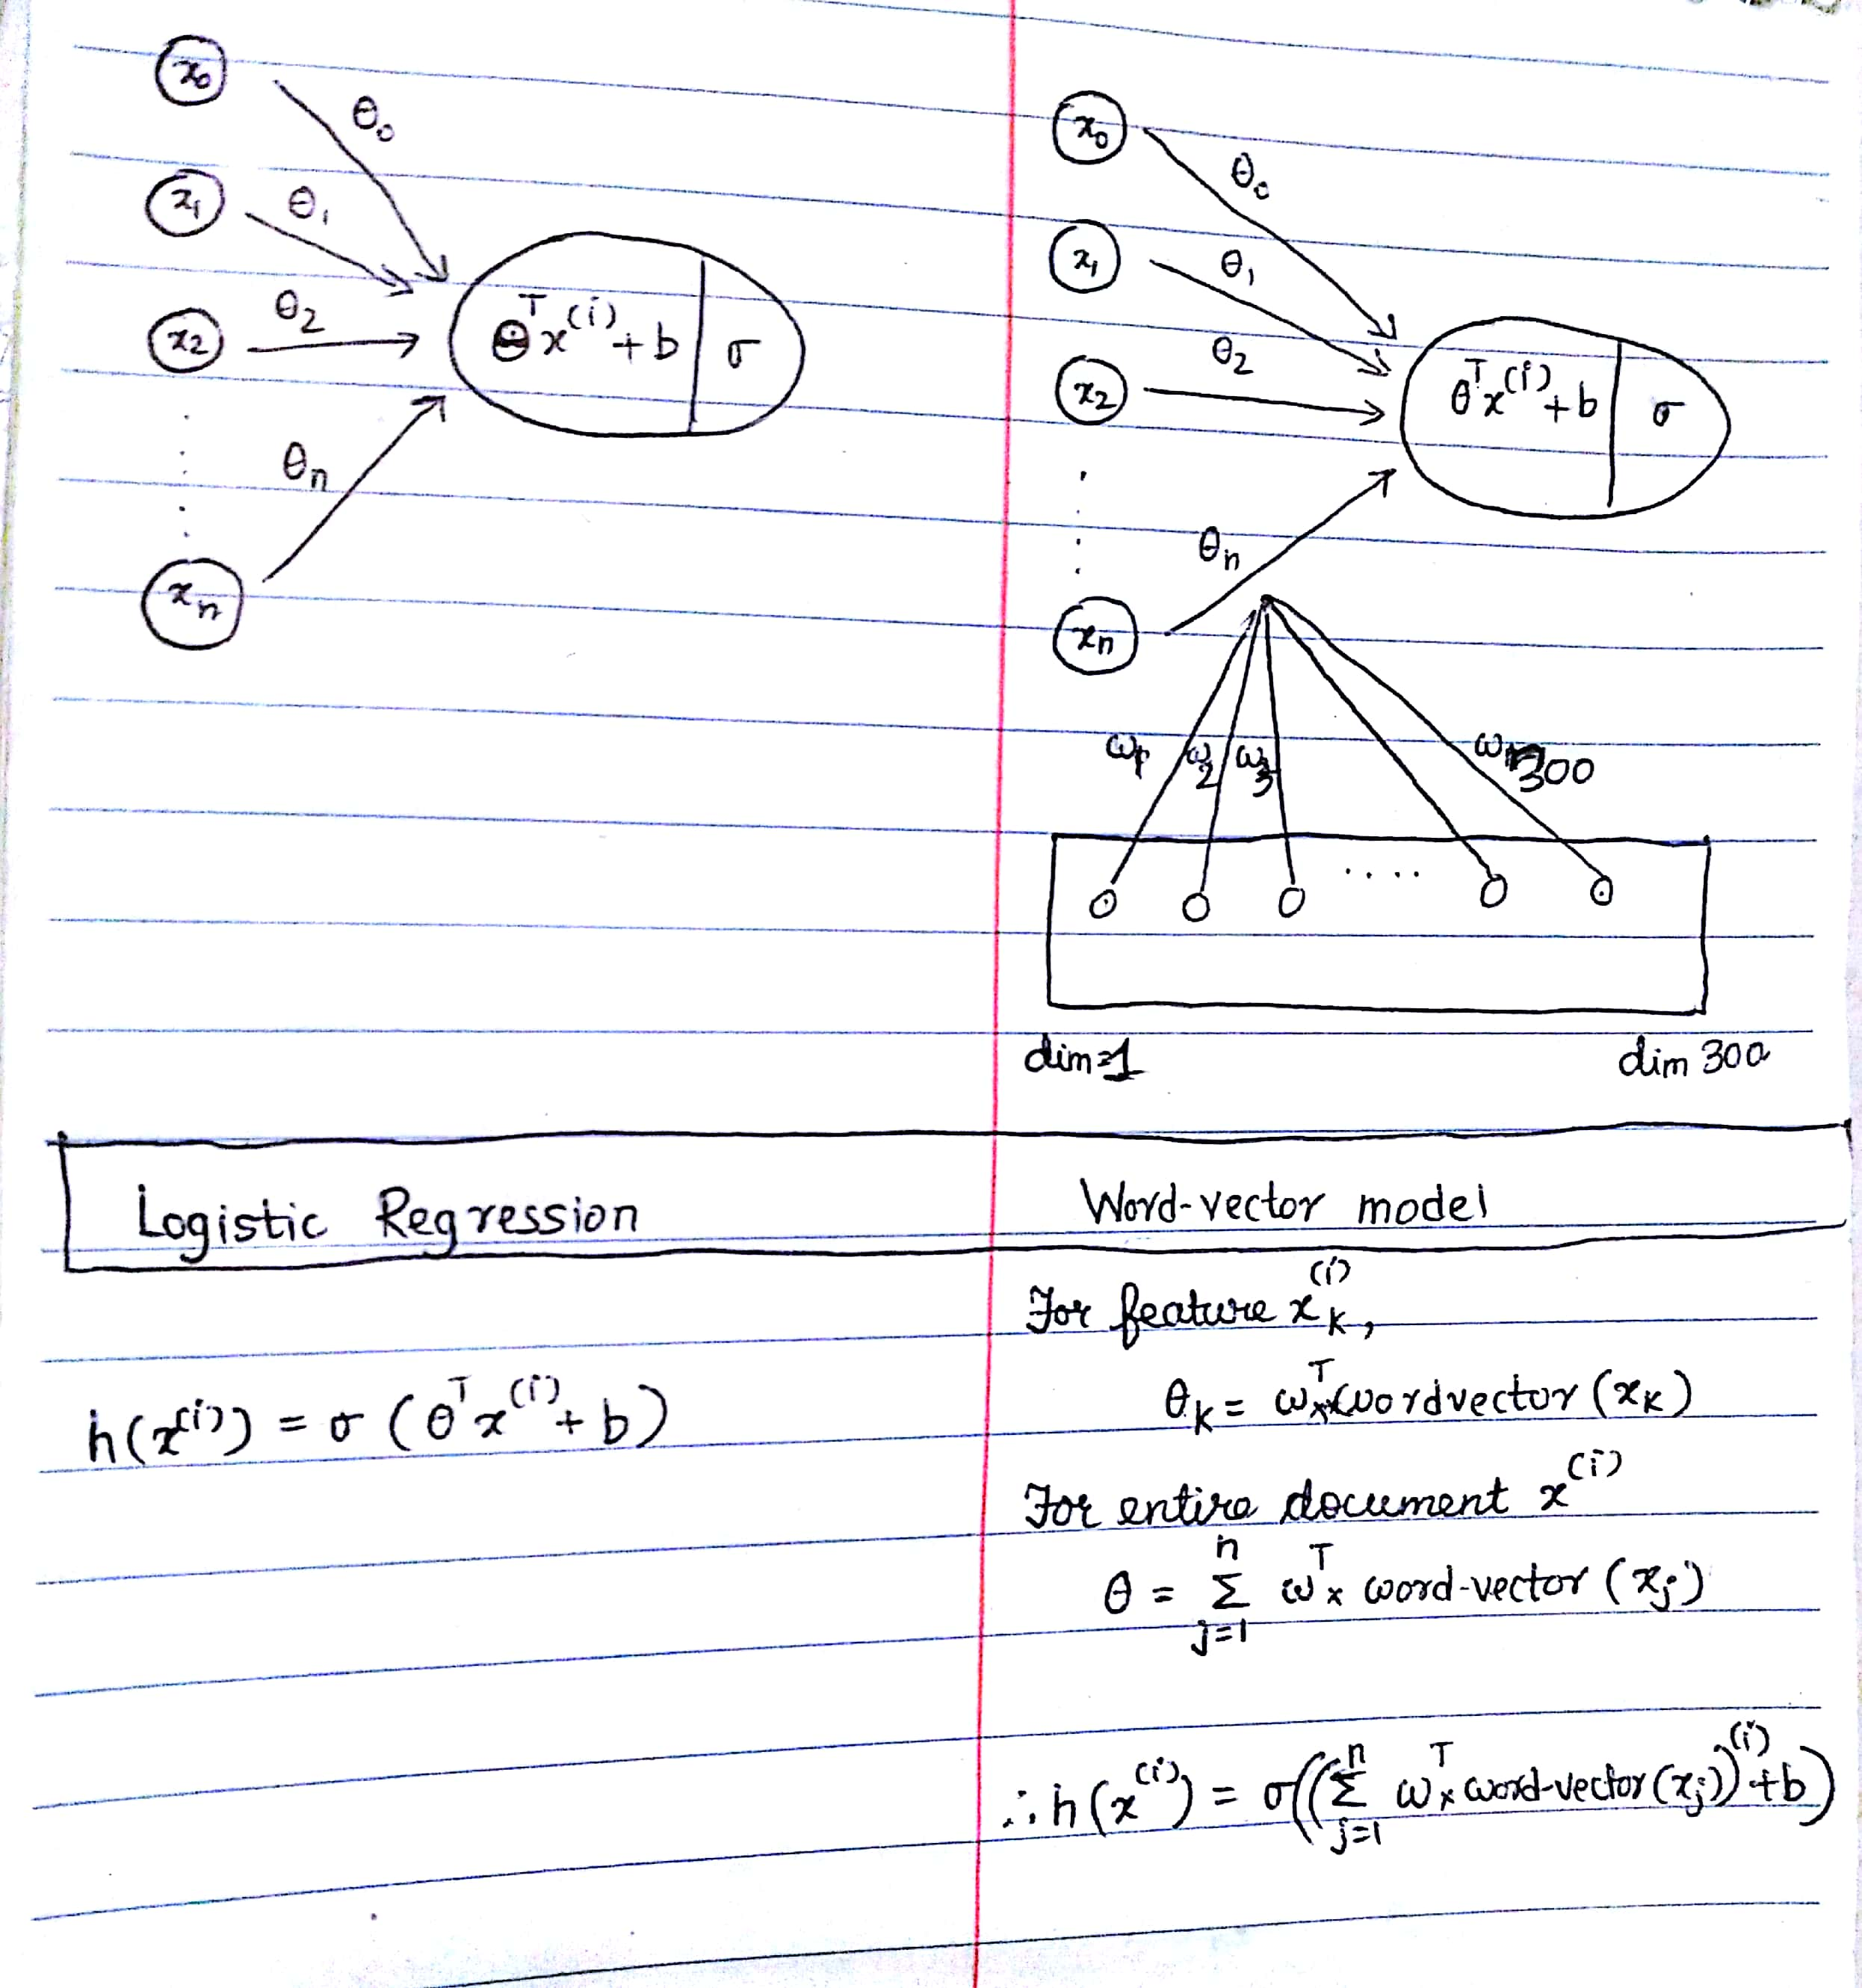
\includegraphics[width=16cm, height=10cm]{wordvec.jpg}\\[1cm]
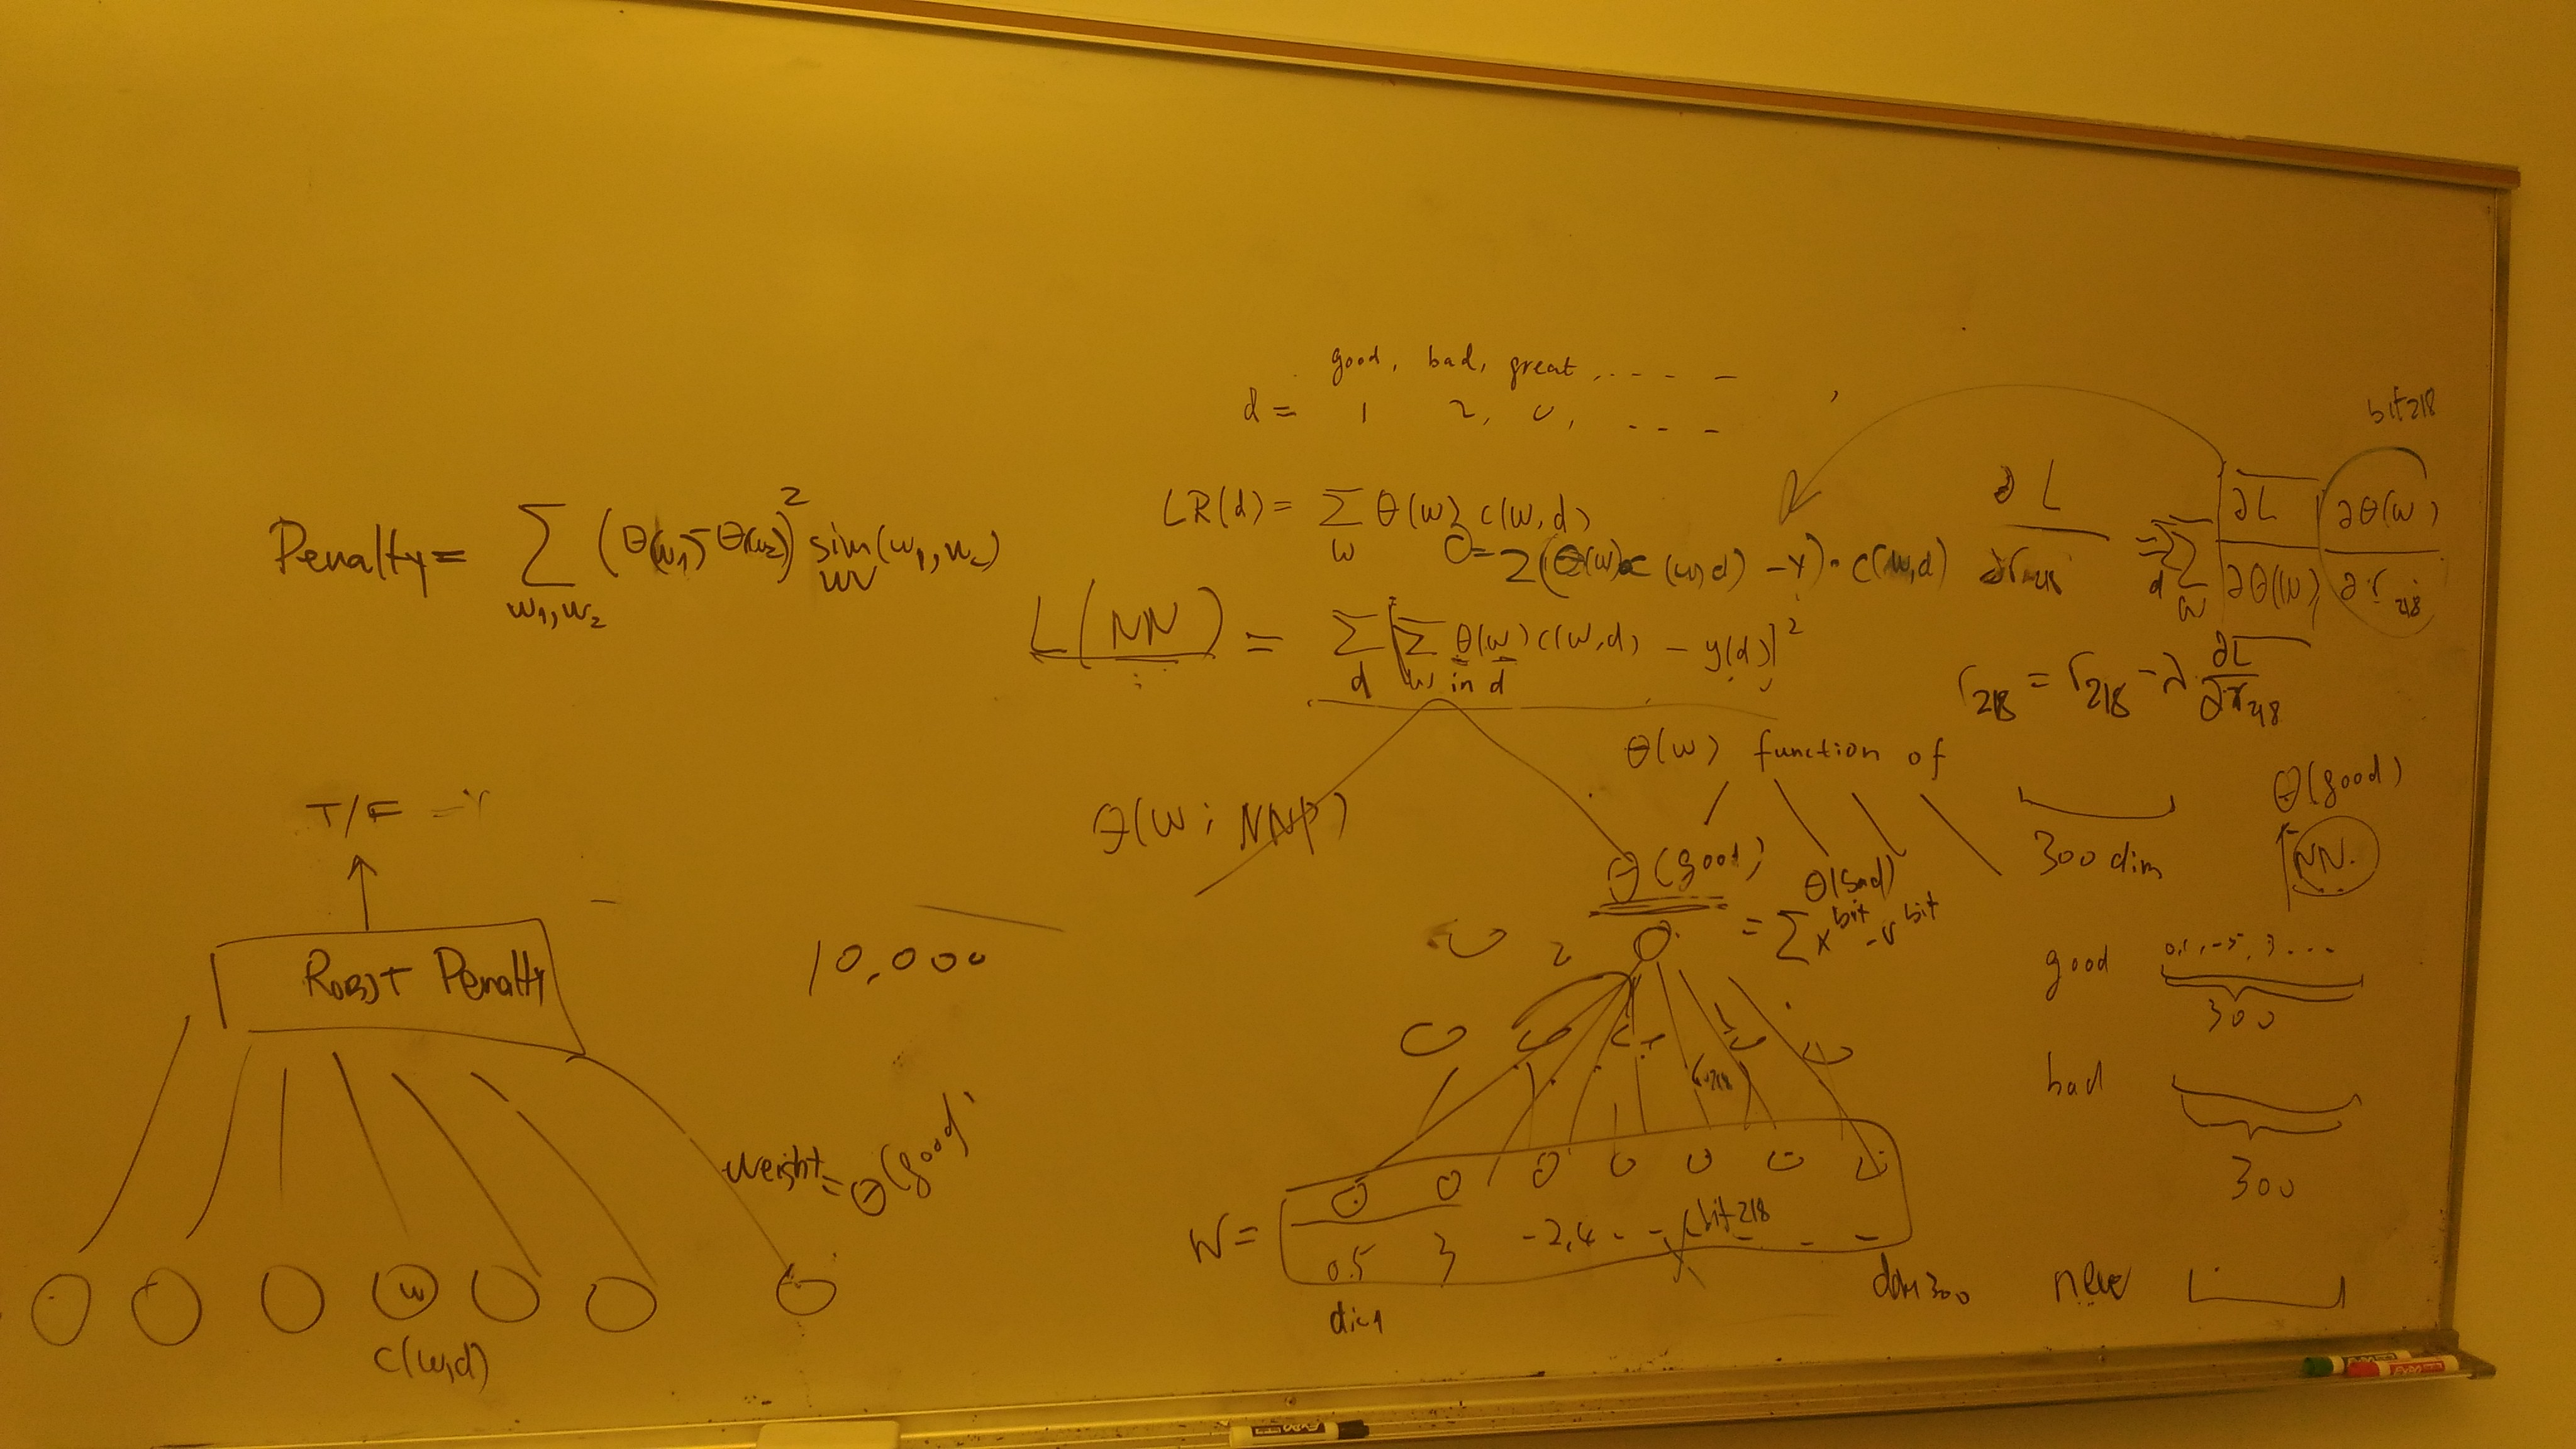
\includegraphics[width=16cm, height=10cm]{cheng.jpg}\\[1cm]

\end{document}